\documentclass[11pt]{article}
\usepackage{anysize} 
\marginsize{2cm}{2cm}{2cm}{2cm} 

\usepackage{multirow}
\usepackage{tabularx}
\usepackage{longtable}
\usepackage[utf8]{inputenc}
\usepackage[spanish]{babel}
\usepackage{hyperref}
\usepackage{fixltx2e}
\usepackage{mathtools}
\usepackage{amsmath}
\usepackage{graphicx}
\usepackage{adjustbox}
\usepackage{subcaption}

%%%%%%%%%%%%%%%%%%%%%%%%%%%%%%%%%%%%%%%%%%%%%%%%%
%	headers & footers							%
%%%%%%%%%%%%%%%%%%%%%%%%%%%%%%%%%%%%%%%%%%%%%%%%%
\usepackage{fancyhdr}
\pagestyle{fancy}
\fancyhf{}
\rhead{Taller de Sistemas Computacionales}
\lhead{Segundo Semestre 2014}
\rfoot{Página \thepage}

%%%%%%%%%%%%%%%%%%%%%%%%%%%%%%%%%%%%%%%%%%%%%%%%%
%	comandos									%
%%%%%%%%%%%%%%%%%%%%%%%%%%%%%%%%%%%%%%%%%%%%%%%%%

\newcommand{\labno}{2}
\newcommand{\labtitle}{Taller de Sistemas Computacionales}
\newcommand{\nameone}{Iván González López}
\newcommand{\emailone}{ivan.gonzalezlo@alumnos.usm.cl}
\newcommand{\rolone}{2973523-9}
\newcommand{\nametwo}{Guillermo Baeza Figueroa}
\newcommand{\emailtwo}{guillermo.baeza@alumnos.usm.cl}
\newcommand{\roltwo}{2973600-6}

\begin{document}
\begin{titlepage}
\begin{center}

%%%%%%%%%%%%%%%%%%%%%%%%%%%%%%%%%%%%%%%%%%%%%%%%%
%	título página inicial						%
%%%%%%%%%%%%%%%%%%%%%%%%%%%%%%%%%%%%%%%%%%%%%%%%%


\includegraphics[width=70pt]{logos/utfsm.pdf} \\
{\Large \textsc{Universidad Técnica Federico Santa María} \\}
{\Large \textsc{Departamento de Informática} \\ \vspace{4pt}}
{\rule[13pt]{\textwidth}{1pt} \\ \vspace{25pt}}
{\LARGE \textsc{Tarea No. \labno} \\}
{\LARGE \textsc{\labtitle} \\ \vspace{50pt}}

%%%%%%%%%%%%%%%%%%%%%%%%%%%%%%%%%%%%%%%%%%%%%%%%%
%	autores										%
%%%%%%%%%%%%%%%%%%%%%%%%%%%%%%%%%%%%%%%%%%%%%%%%%
\begin{minipage}{0.4\textwidth}
\begin{flushleft}
{\large \nameone} \\
\emailone \\
\rolone
\end{flushleft}
\end{minipage}
\hfill
\begin{minipage}{0.4\textwidth}
\begin{flushright}
{\large \nametwo} \\
\emailtwo \\
\roltwo
\end{flushright}
\end{minipage}
\end{center}
\end{titlepage}


\section{Descripción}
Para este segundo informe, realizamos la conexión a través de un servidor de máquinas virtuales a las máquinas que habían sido previamente creadas, las que tienen dos versiones distintas de Linux CentOs: una versión desktop (full) y otra servidor mínimo (sin entorno gráfico).\par
El trabajo consistió en realizar un primer acercamiento al sistema CentOs, por lo que lo primero fue configurar las cuentas de usuario y posteriormente verificar algunos parámetros de red. El desarrollo de todo esto se encuentra en la siguiente sección.
\section{Análisis y Desarrollo}
\subsection{Configuración de cuenta de usuario}
Una vez iniciadas las máquinas virtuales con las dos versiones de CentOs instaladas, lo primero fue cambiar las contraseñas de las cuentas root y TSC, de las versiones de servidor y desktop respectivamente. Esto se realiza en ambas versiones con un mismo comando \textit{passwd} en consola.\par
\textit{Notar que se nos advierte que la contraseña escogida es demasiado trivial, pero aun así se nos permite utilizarla.}\\
	
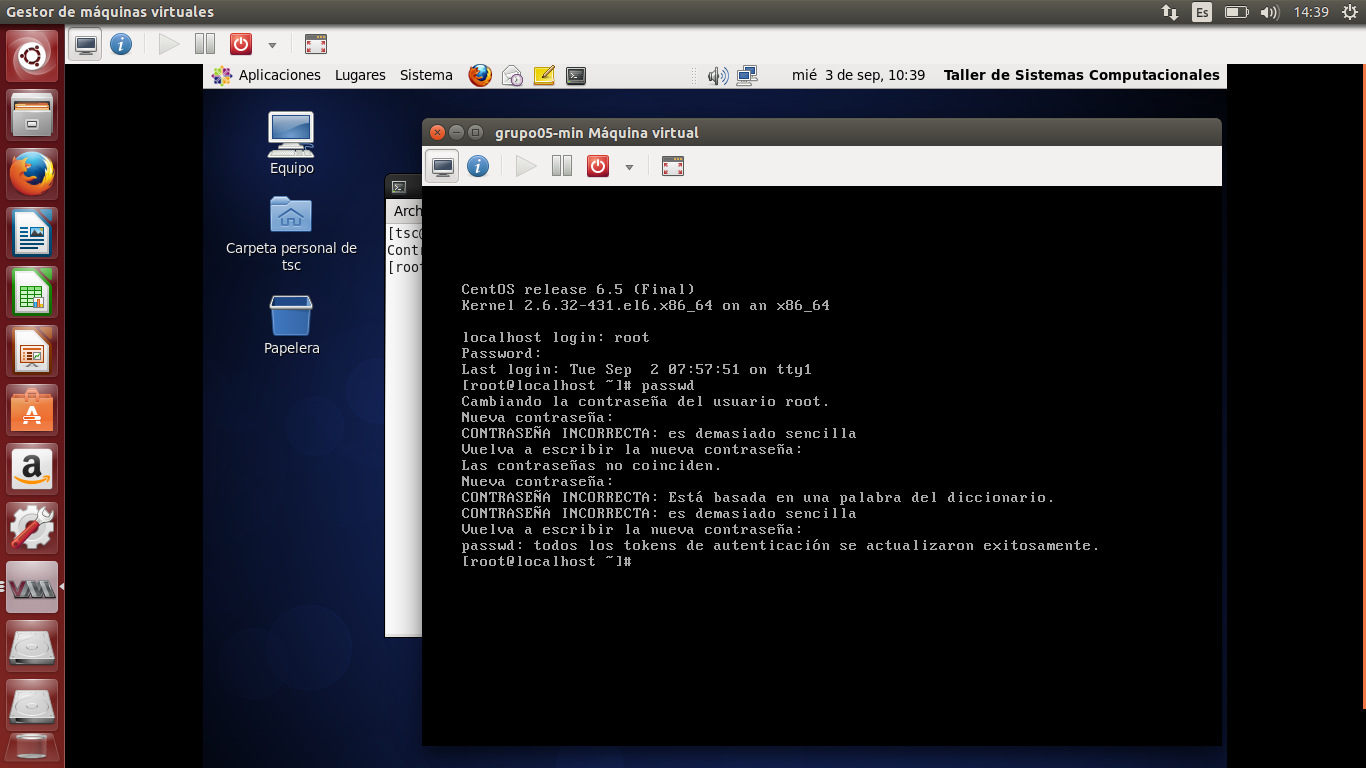
\includegraphics[width=.75\linewidth]{screenshots/minimal/passwd.png}
    \\Comando \textit{passwd} para cambiar contraseña de root en versión mínima.\\

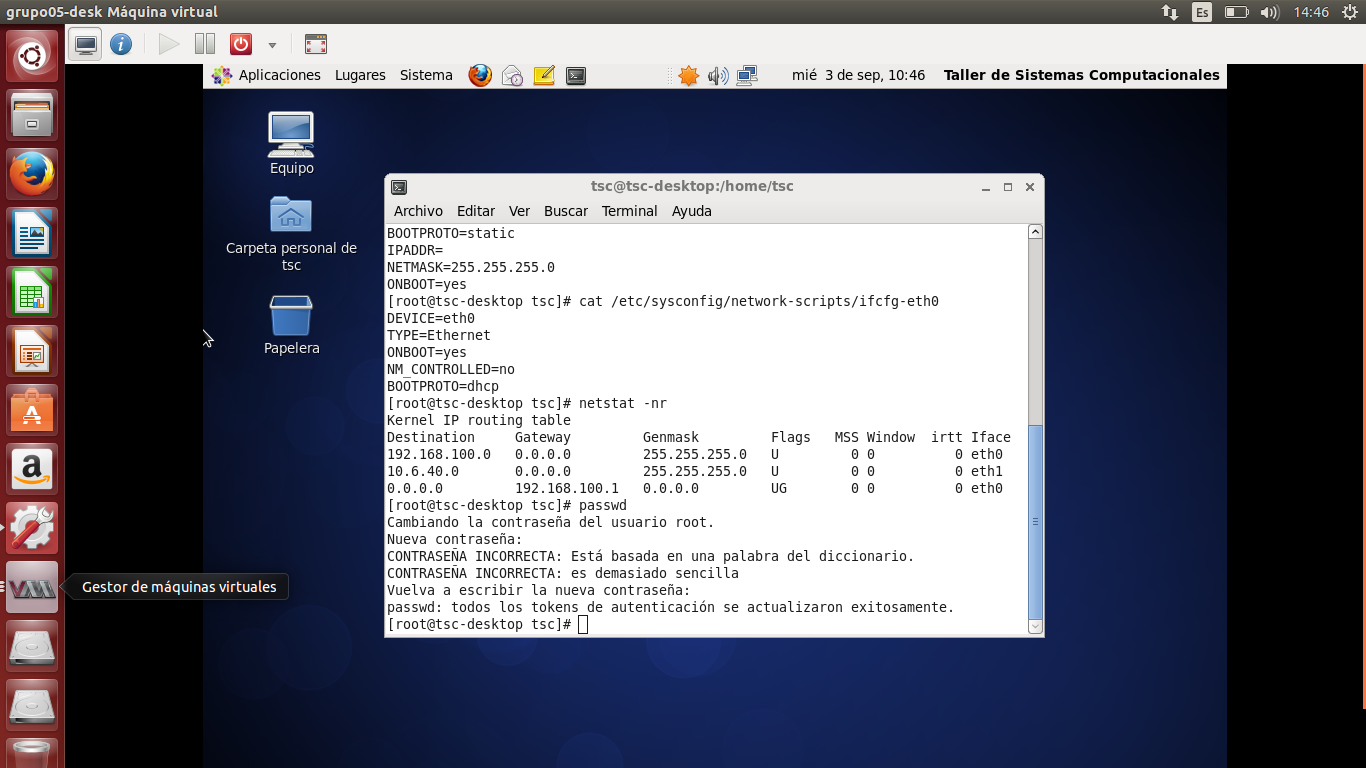
\includegraphics[width=.75\linewidth]{screenshots/desktop/passwd.png}
    \\Comando \textit{passwd} para cambiar contraseña de root en versión desktop.\\
\newpage
\subsection{Recopilación de datos de red}
\subsubsection{IP}
De manera análoga a la primera experiencia desarrollada en nuestros computadores personales, fue necesario configurar algunos parámetros de red. Primero, se editó el archivo ubicado en \textbf{/etc/sysconfig/network-scrips/eth1} para configurar manualmente la IP de la máquina virtual. En el caso de la versión mínima, la IP configurada fue \textbf{10.6.40.225} mientras que la IP configurada en la versión desktop fue \textbf{10.6.40.195}.\\

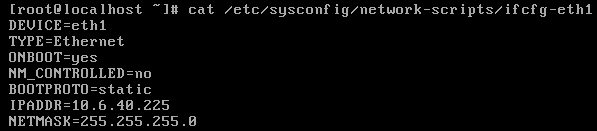
\includegraphics[width=.75\linewidth]{screenshots/minimal/cat-ifcfg-eth1.png}
    \\Configuración de IP en versión mínima.\\

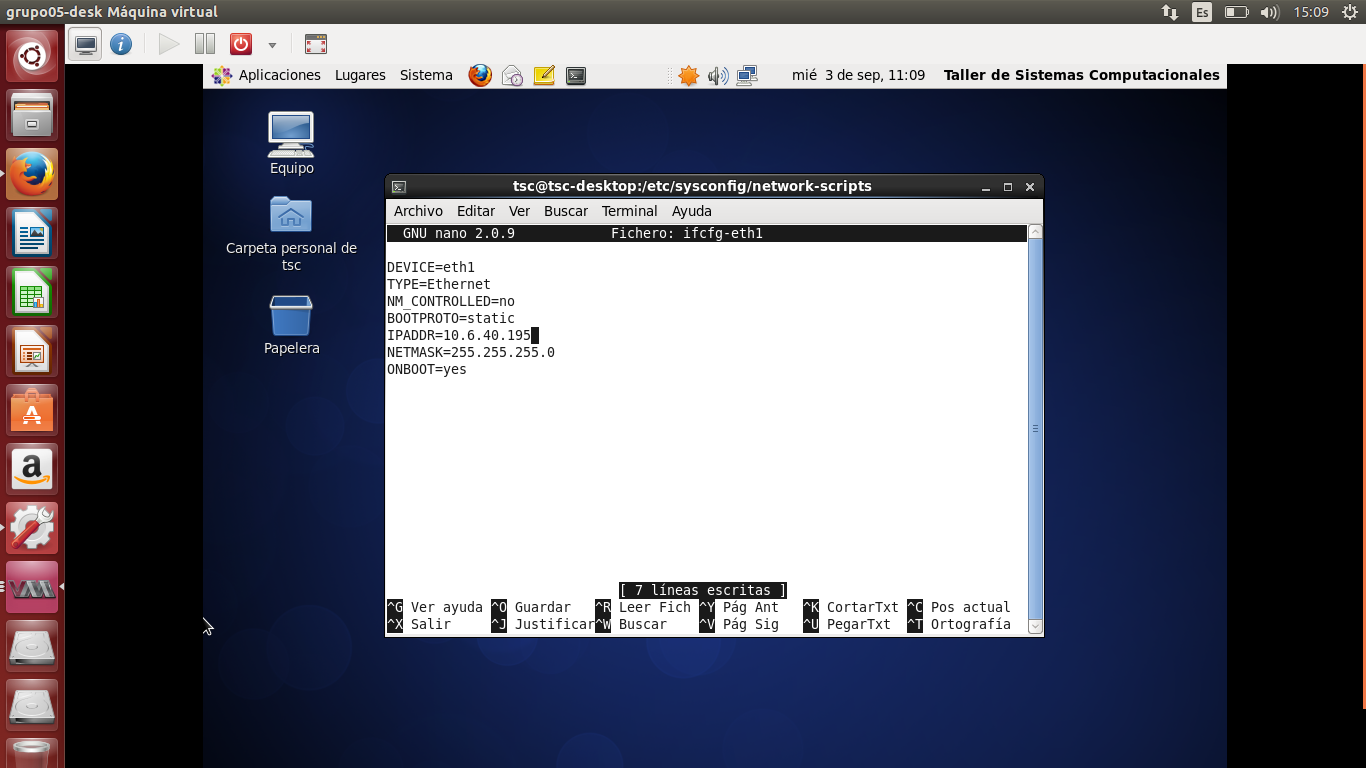
\includegraphics[width=.75\linewidth]{screenshots/desktop/ifcfg-eth1.png}
    \\Configuración de IP en versión desktop.\\
    
Por otro lado, dentro de la misma carpeta, en el archivo \textbf{eth0} fue necesario cambiar el valor binario de NM\_CONTROLLED a \textit{yes}, de esta manera la gestión de la interfaz de red es llevada a cabo por el NetworkManager.\\

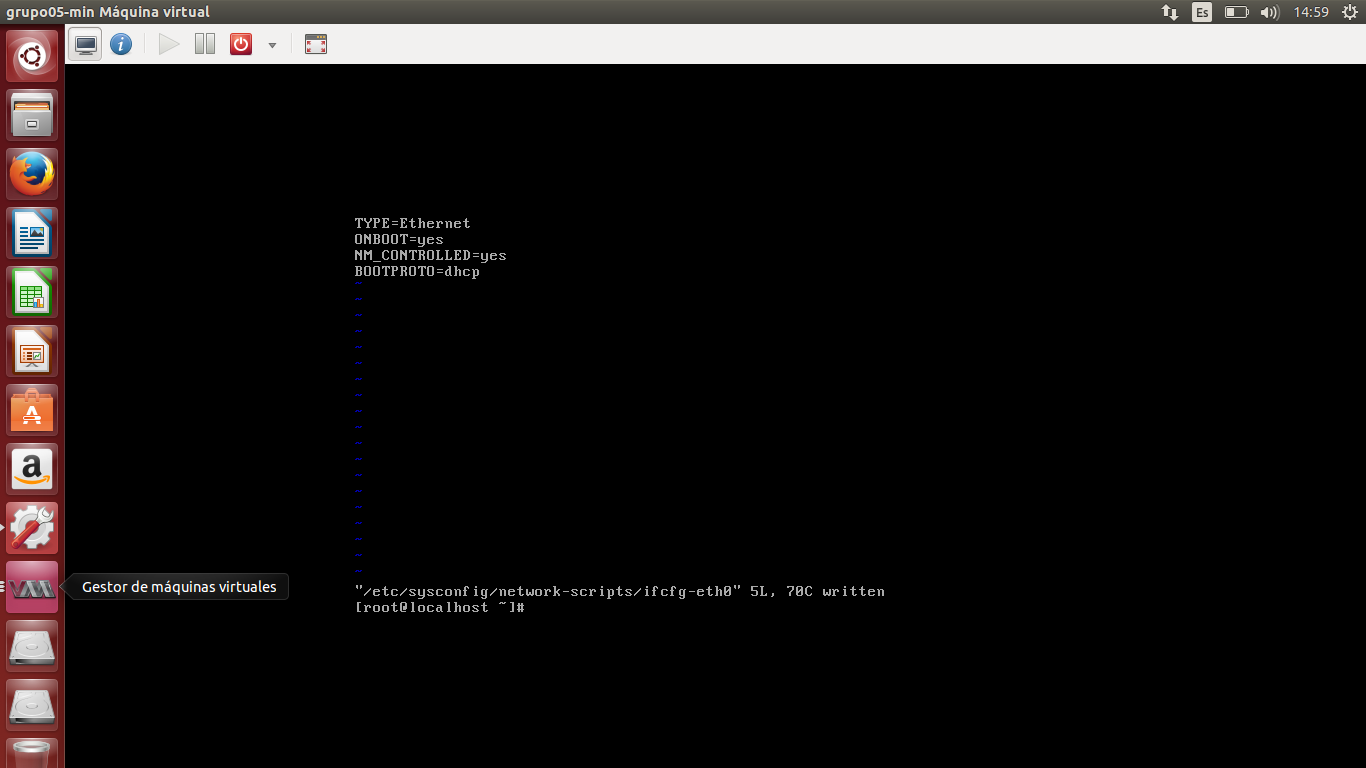
\includegraphics[width=.75\linewidth]{screenshots/minimal/ifcfg-eth0(after).png}
    \\Configuración de NetworkManager en versión mínima.\\

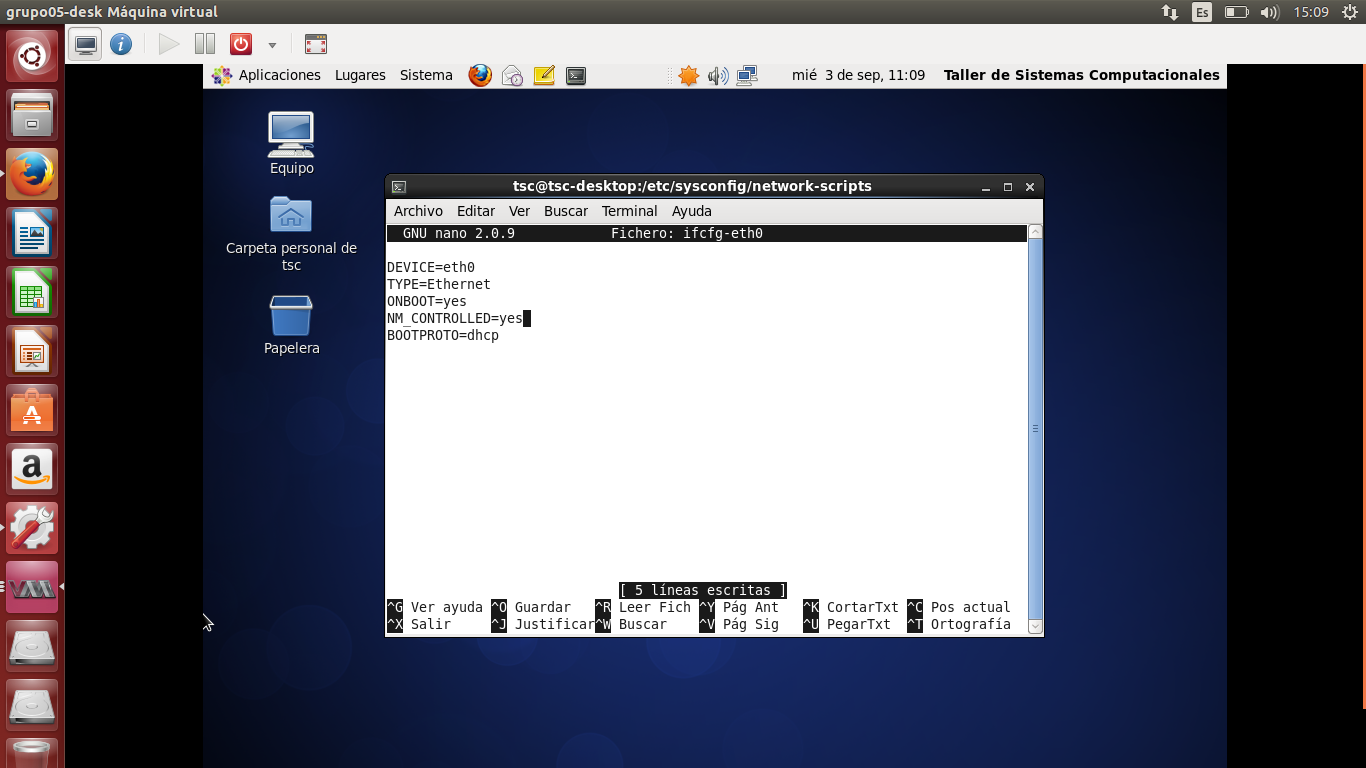
\includegraphics[width=.75\linewidth]{screenshots/desktop/ifcfg-eth0.png}
    \\Configuración de NetworkManager en versión desktop.\\
\newpage
\subsubsection{DNS}
	En esta parte había que ver el contenido del archivo \textbf{/etc/resolv.conf} usado para resolver el nombre de los servidores en internet. Para ello, hacemos un simple comando \textit{cat}, en ambas versiones de CentOS.\\
	
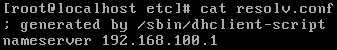
\includegraphics[width=.45\linewidth]{screenshots/minimal/cat-resolv-conf.png}
    \\Contenido archivo \textit{resolv.conf} en versión mínima.\\

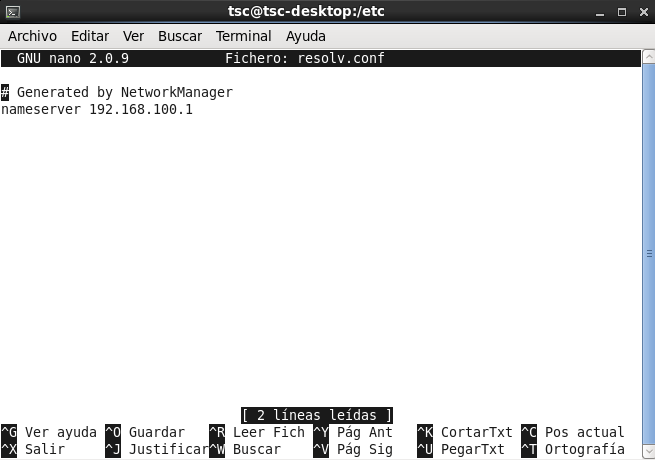
\includegraphics[width=.75\linewidth]{screenshots/desktop/resolv-conf.png}
    \\Contenido archivo \textit{resolv.conf} en versión desktop.
\newpage
\subsubsection{Puerta de enlace}
	Luego, fue necesario verificar la puerta de enlace (\textit{default gateway}) de las máquinas. Ello puede hacerse a través de un simple comando \textit{route} en ambas versiones de CentOs.\\

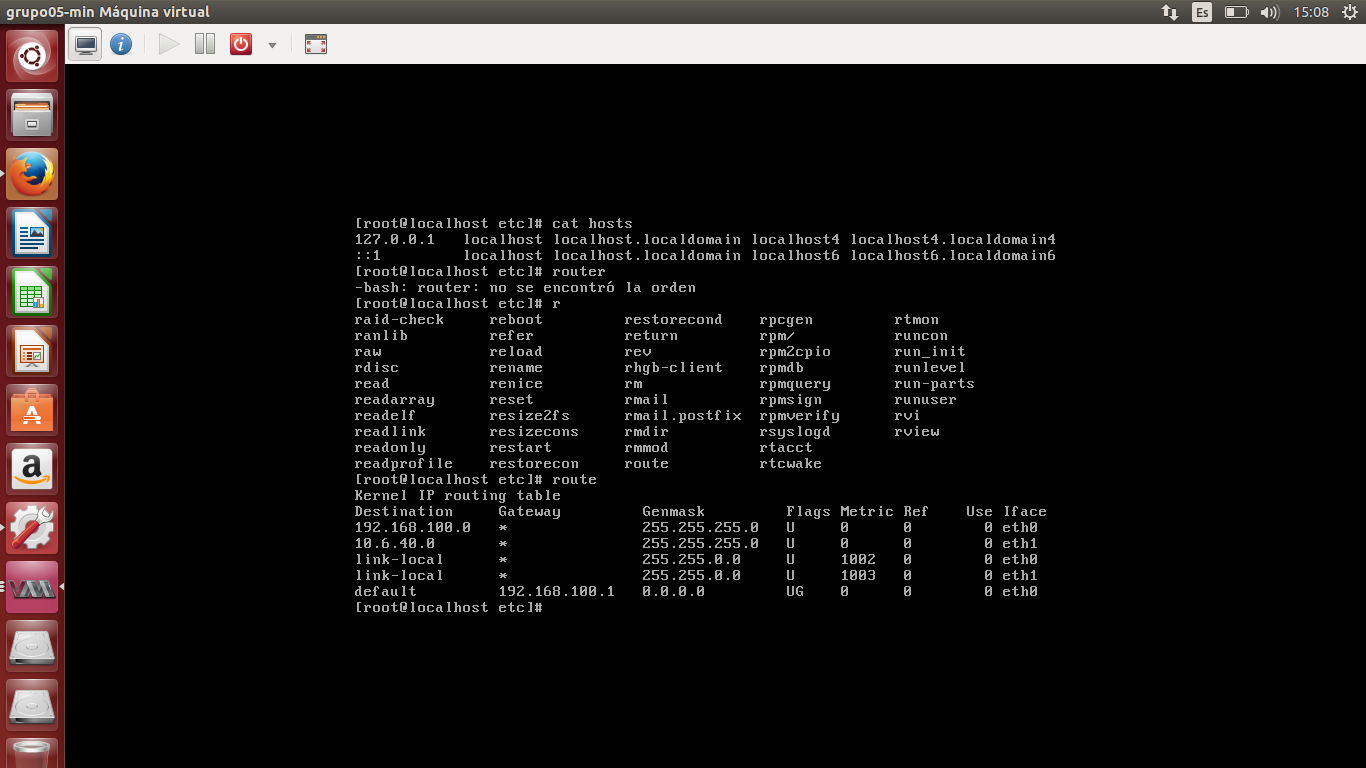
\includegraphics[width=.75\linewidth]{screenshots/minimal/route.png}
    \\Puerta de enlace en versión mínima.\\

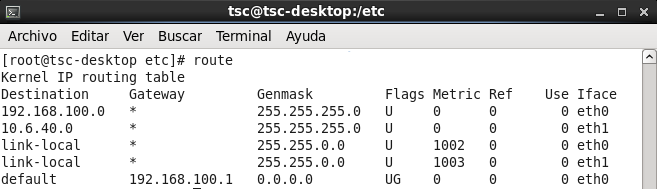
\includegraphics[width=.75\linewidth]{screenshots/desktop/route.png}
    \\Puerta de enlace en versión desktop.
\newpage
\subsubsection{Otros}
    Finalmente, para comprobar que todo estuviera en orden y funcionando correctamente, se hace un ping bidireccional, vale decir, un ping desde la máquina virtual con CentOs minimal a la máquina con CentOs desktop y otro en sentido inverso.\\
    
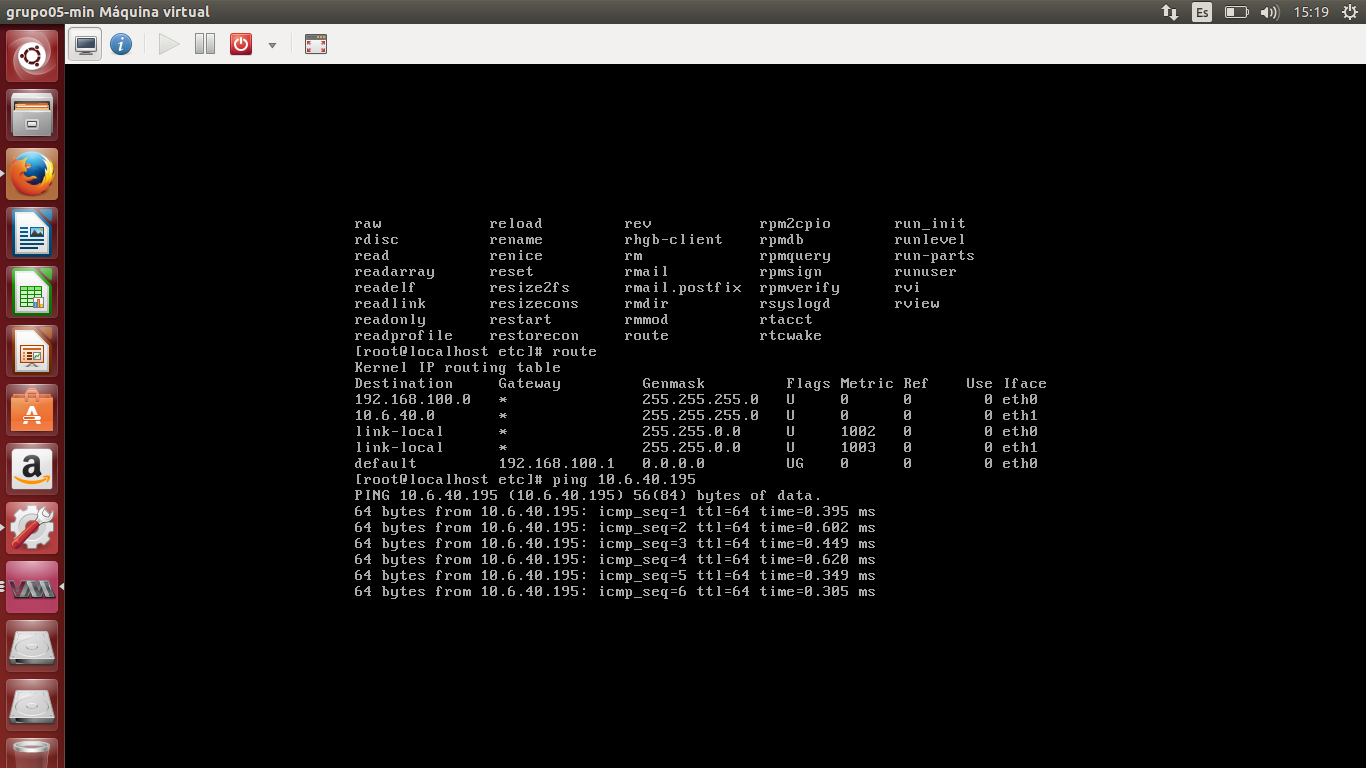
\includegraphics[width=.75\linewidth]{screenshots/minimal/ping-to-desktop.png}
    \\Ping desde la máquina con CentOs desktop hacia la con versión desktop.\\
    
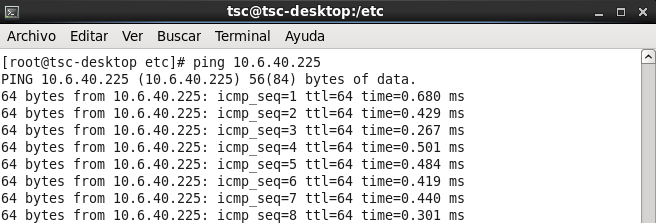
\includegraphics[width=.75\linewidth]{screenshots/desktop/ping-to-min.png}
    \\Ping desde la máquina con CentOs desktop hacia la con versión mínima.\\    
    
    Además, se hace un ping a la máquina del profesor cuya IP es \textbf{10.6.40.245}, desde nuestra máquina con CentOS minimal.\\
    
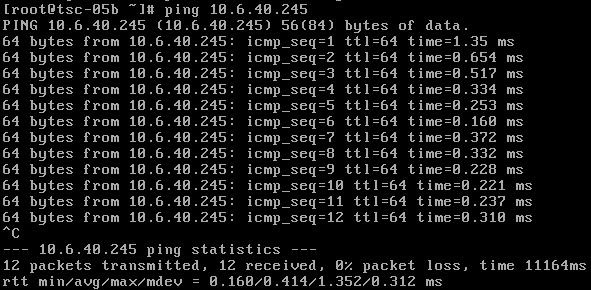
\includegraphics[width=.75\linewidth]{screenshots/minimal/ping-to-profe.png}
    \\Ping desde la máquina con CentOs minimal hacia la del profesor.\\    
\end{document}
